In this section we provide details about ESMACS and TIES specifications and
about adaptive methodologies using TIES\@. We conclude with a description and
validation of the physical systems used in this work.

% ---------------------------------------------------------------------------
\subsection{ESMACS and TIES}\label{ssec:esm_ties}

ESMACS and TIES~\cite{Wan2017brd4, Bhati2017} are two free energy calculation
protocols that implement absolute and relative methods, respectively.
Absolute free energy methods calculate the binding affinity of a
\emph{single} drug molecule to a protein, while relative methods calculate
the \emph{difference} in binding affinity between two (usually similar in
structure) drug molecules. Both protocols are designed to use an ensemble MD
simulation approach to enhance the reproducibility and accuracy of standard
free energy calculation techniques (MMPBSA~\cite{Massova1999} in the case of
ESMACS and thermodynamic integration~\cite{Straatsma1988, Straatsma1991} in
TIES). The use of ensemble averaging allows tight control of error bounds in
the resulting free energy estimates.

ESMACS and TIES consists of three main steps: minimization, equilibration and
production MD (in its current implementation all MD steps are conducted in
NAMD~\cite{Phillips2005}). In practice, the equilibration phase is broken
into multiple steps to ensure that the size of the simulation box does not
alter too much over the simulation. During these steps, positional
constraints are gradually released from the structure and the physical system
is heated to a physiologically realistic temperature.

Whilst both protocols share a common sequence of steps, the make-up of the
ensemble is different. In ESMACS, an ensemble consists of a set of 25
\textbf{replicas}, i.e., identical simulations differing only in the initial
velocities assigned to each atom. In TIES, the ensemble contains a set of
\textbf{$\lambda$} windows, each spawning a set of replicas. As a
transformation parameter $\lambda$ increases from 0 to 1, the system
description transforms from containing an initial drug to a target compound
via a series of hybrid states. Sampling along $\lambda$ is then required to
compute the difference in binding free energy. In previous studies, TIES has
been deployed using 65 replicas, evenly distributed among 13 $\lambda$
windows. Following the completion of the simulation steps, both protocols
require the execution of free energy analysis steps. The detailed composition
of ESMACS and TIES protocols is shown in
Fig.~\ref{fig:ties_esmacs_application}.

\begin{figure}
  \centering
  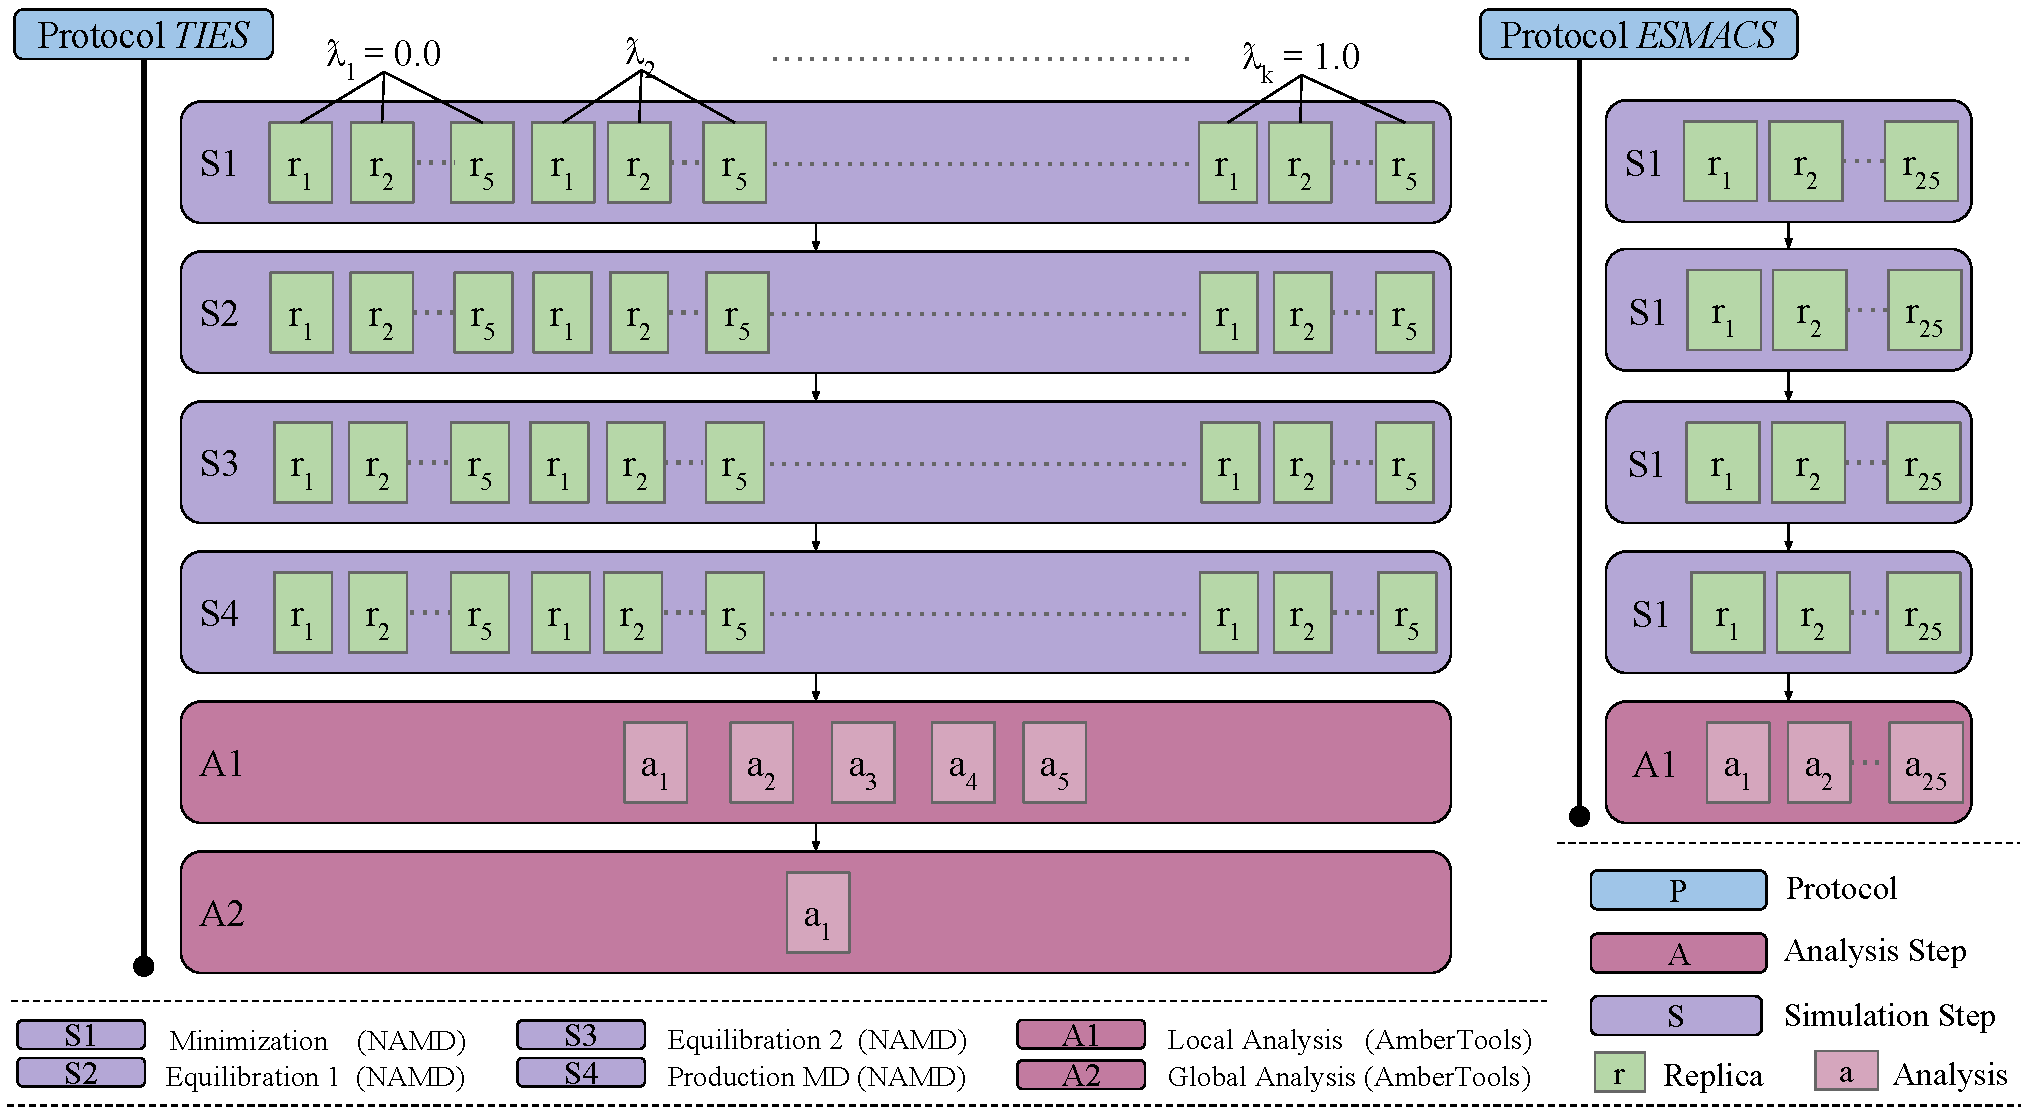
\includegraphics[width=\columnwidth]{figures/ties_esmacs_application_model.pdf}
  \caption{TIES and ESMACS protocols consist of simulations steps followed by
  analysis step(s). ESMACS contains 25 replicas per simulation step; TIES
  contains 5 replicas per $\lambda$ window. We model TIES with 13 $\lambda$
  windows, spawning 65 replicas in each simulation step. All replicas
  simulate 6ns.}\label{fig:ties_esmacs_application}
\up{}
\up{}
\end{figure}

% ---------------------------------------------------------------------------
\subsection{The Value of Adaptivity}\label{ssec:adapt_ties}

The main driver for adaptivity is that computational campaigns will typically
involve compounds with a wide range of chemical properties which can impact
the time to convergence and the type of sampling required to gain accurate
results. There may be cases where it is important to increase the sampling of
phase space, possibly through expanding the ensemble. In general, there is no
way to know exactly which calculation setup a particular system requires
before runtime.

Another driver of adaptivity is that, on occasion, alchemical methods may
converge very slowly. This means that the most effective way to gain accurate
and precise free energy results on industrially or clinically relevant
timescales is to adapt either the workflow corresponding to a specific
protocol or adapt different workflows in relation to each other. The latter is
referred to as \textbf{inter-protocol} adaptivity; the former as
\textbf{intra-protocol} wherein, for example, the parameter values associated
with a specific protocol might change. With thousands of workflows
(corresponding to a protocol instances) to adapt in different ways, this has
the potential to allow for significant optimization.

% simulations, often employing multiple analysis methodologies, this provides
% the most effective way to utilize these techniques and resources at scale.

In TIES, the change in free energy associated with the transformation is
calculated using an adaptive quadrature function which numerically integrates
the values of the $\partial U/\partial\lambda$ across the full set of
simulated $\lambda$ windows. Obtaining accurate and precise results from TIES
using adaptive quadratures requires that the $\lambda$ windows correctly
capture the changes of $\partial U/\partial\lambda$ over the transformation.
This behavior is highly sensitive to the chemical details of the compounds
being studied and varies considerably among candidates. Typically, $\lambda$
windows are evenly spaced between 0 and 1 with the spacing between them set
before execution at a distance determined by the simulator to be sufficient
for a wide range of systems.

However, the number or the location of the $\lambda$ windows that will most
impact the calculation are not known \textit{a priori}, and varies across
candidates. As each window requires multiple simulations, sampling with a
high frequency is expensive. Approximations using evenly spaced $\lambda$
windows reach an acceptable accuracy threshold but adaptive placement of
$\lambda$ windows is likely to better capture the shape of the $\partial
U/\partial\lambda$ curve, leading to more accurate and precise results for a
comparable computational cost.

% we use adaptive middleware to automate runtime decisions based
% on partial simulation data, and redistribute resources at runtime to support
% dynamically generated simulations. We

In this work, we focus on intra-protocol adaptivity
which relies on intermediate runtime results \textit{within} a protocol
instance to define the following set of simulations. Instead of approximating
the placement of all the $\lambda$ windows prior to execution, we run TIES
with less $\lambda$ windows and shorter bursts of simulations, analyzing
intermediate runtime results (i.e., trajectories) to seed new and ideally
placed $\lambda$ windows.